\section{Background}
\subsection{SDN}
An SDN-enabled network provides a \textit{Controller} unit or system that comprises the control
logic of the network devices located on separate computer resources resulting in the differentiation
between the so called \textit{data-} and \textit{control-plane}. It features a \textit{Southbound
API} for conveying information \emph{down} to the devices in the data plane as well as a
\textit{Northbound API} for communication with application and business logic \emph{up top}.

SDN Controllers thus provide a centralized view on the network and could potentially be used to
retrieve information for utilization by the data processing platform in deployment decisions.
Furthermore, the functions available for network manipulation could be invoked during runtime based
on the knowledge about currently running analytical jobs.

\subsection{Apache Flink}
For this paper, we used Apache Flink as our data processing engine. Flink is a \textit{Fast and
Reliable Large-Scale Data Processing engine}. A Flink cluster can be made up from a number of
physical computation nodes or even a single host. Processing programs, written in Java or Scala by
the user, are automatically adapted by the optimizer and runtime to execute efficient on a given
setup.\footnote{(2015) Apache Flink home. Retrieved March 20, 2015, from https://flink.apache.org}
The result of this adaption is the so-called \textit{Execution Graph}, which is deployed. A
master-node, the \textit{Job Manager} is responsible for doing so and keeping track of the the
overall job execution. The job is split up into several tasks that can be handled independant by
\textit{Task Managers} - the actual computation nodes. Depending on the physical hardware, a task
manager can offer multiple processing slots. A sketch of the scheduling is depicted in Figure
\ref{fig:job_execution} and \ref{fig:embedding}.

\begin{figure}[h]
    \centering
    \begin{minipage}{0.5\textwidth}
        \centering
        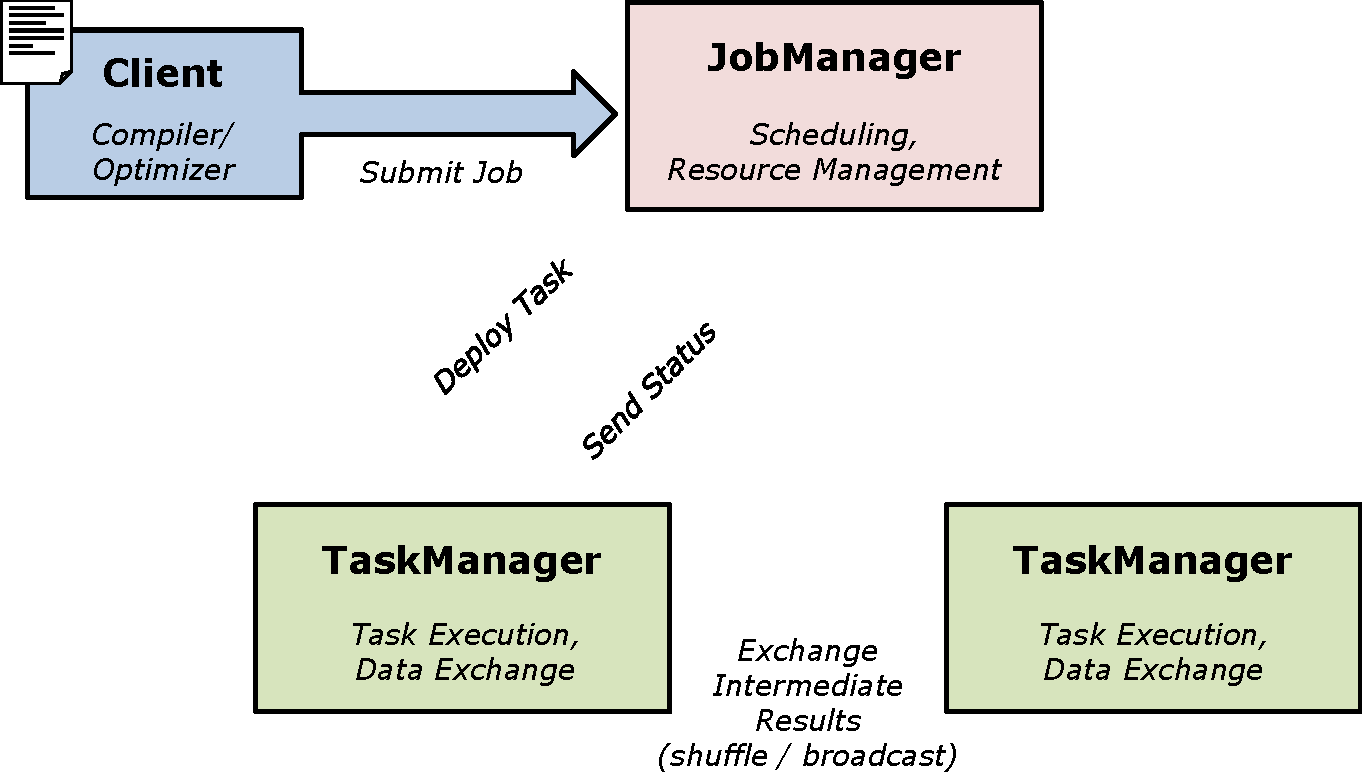
\includegraphics[width=1.0\linewidth]{graphics/ClientJmTm.pdf}
        \captionof{figure}{Sketch of Job Execution\protect\footnotemark}
        \label{fig:job_execution}
    \end{minipage}%
    \begin{minipage}{0.5\textwidth}
        \centering
        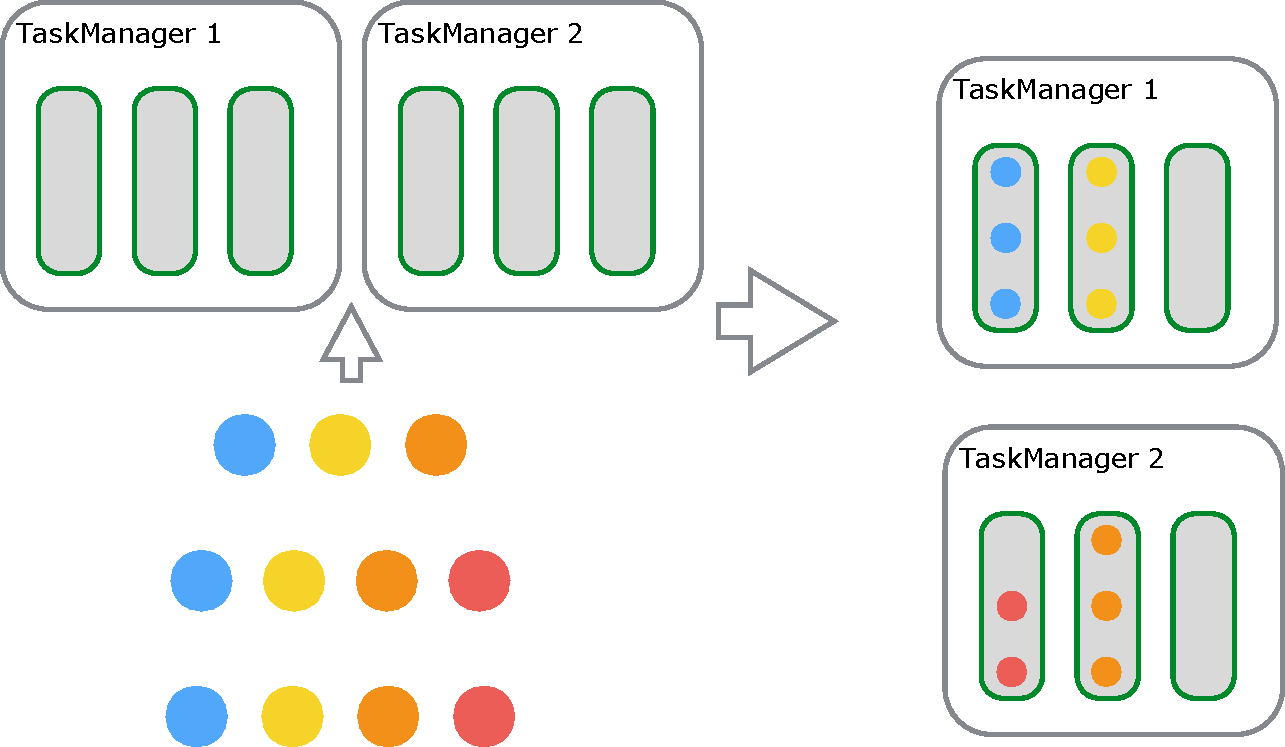
\includegraphics[width=1.0\linewidth]{graphics/slots.pdf}
        \captionof{figure}{Execution-Graph embedding to Task Managers\protect\footnotemark}
        \label{fig:embedding}
    \end{minipage}
\end{figure}

% fix to reference the previous footnotemark
\addtocounter{footnote}{-1}
\footnotetext{(2015) ClientJmTm.svg Github/Apache/Flink-master from
https://raw.githubusercontent.com/apache/flink/master/docs/img/ClientJmTm.svg}
\stepcounter{footnote}
\footnotetext{(2015) Slots.svg Github/Apache/Flink-master from
https://raw.githubusercontent.com/apache/flink/master/docs/img/slots.svg}

